% This file was created with tikzplotlib v0.9.14.
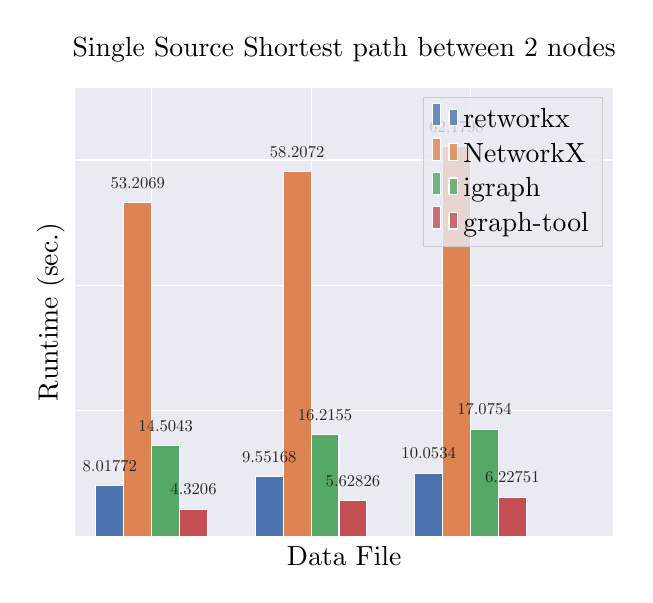
\begin{tikzpicture}

\definecolor{color0}{rgb}{0.917647058823529,0.917647058823529,0.949019607843137}
\definecolor{color1}{rgb}{0.298039215686275,0.447058823529412,0.690196078431373}
\definecolor{color2}{rgb}{0.866666666666667,0.517647058823529,0.32156862745098}
\definecolor{color3}{rgb}{0.333333333333333,0.658823529411765,0.407843137254902}
\definecolor{color4}{rgb}{0.768627450980392,0.305882352941176,0.32156862745098}

\begin{axis}[
axis background/.style={fill=color0},
axis line style={white},
legend cell align={left},
legend style={fill opacity=0.8, draw opacity=1, text opacity=1, draw=white!80!black, fill=color0},
tick align=outside,
title={Single Source Shortest path between 2 nodes},
x grid style={white},
xlabel={Data File},
xmajorgrids,
xmajorticks=false,
xmin=-0.485, xmax=2.9,
xtick style={color=white!15!black},
xtick={0,1,2},
xticklabels={USA-road-1.USA,USA-road-d.USA,USA-road-t.USA},
y grid style={white},
ylabel={Runtime (sec.)},
ymajorgrids,
ymajorticks=false,
ymin=0, ymax=71.5067908215523,
ytick style={color=white!15!black}
]
\draw[draw=white,fill=color1] (axis cs:-0.35,0) rectangle (axis cs:-0.175,8.01772065162659);
\addlegendimage{ybar,ybar legend,draw=white,fill=color1}
\addlegendentry{retworkx}

\draw[draw=white,fill=color1] (axis cs:0.65,0) rectangle (axis cs:0.825,9.55167670249939);
\draw[draw=white,fill=color1] (axis cs:1.65,0) rectangle (axis cs:1.825,10.0533518791199);
\draw[draw=white,fill=color2] (axis cs:-0.175,0) rectangle (axis cs:0,53.2068955421448);
\addlegendimage{ybar,ybar legend,draw=white,fill=color2}
\addlegendentry{NetworkX}

\draw[draw=white,fill=color2] (axis cs:0.825,0) rectangle (axis cs:1,58.2071847915649);
\draw[draw=white,fill=color2] (axis cs:1.825,0) rectangle (axis cs:2,62.1798181056976);
\draw[draw=white,fill=color3] (axis cs:1.38777878078145e-17,0) rectangle (axis cs:0.175,14.5042677879333);
\addlegendimage{ybar,ybar legend,draw=white,fill=color3}
\addlegendentry{igraph}

\draw[draw=white,fill=color3] (axis cs:1,0) rectangle (axis cs:1.175,16.2154607772827);
\draw[draw=white,fill=color3] (axis cs:2,0) rectangle (axis cs:2.175,17.0754391670227);
\draw[draw=white,fill=color4] (axis cs:0.175,0) rectangle (axis cs:0.35,4.320600938797);
\addlegendimage{ybar,ybar legend,draw=white,fill=color4}
\addlegendentry{graph-tool}

\draw[draw=white,fill=color4] (axis cs:1.175,0) rectangle (axis cs:1.35,5.62825741767883);
\draw[draw=white,fill=color4] (axis cs:2.175,0) rectangle (axis cs:2.35,6.22751021385193);
\draw (axis cs:-0.2625,8.01772065162659) ++(0pt,3pt) node[
  scale=0.6,
  anchor=south,
  text=white!15!black,
  rotate=0.0
]{8.01772};
\draw (axis cs:0.7375,9.55167670249939) ++(0pt,3pt) node[
  scale=0.6,
  anchor=south,
  text=white!15!black,
  rotate=0.0
]{9.55168};
\draw (axis cs:1.7375,10.0533518791199) ++(0pt,3pt) node[
  scale=0.6,
  anchor=south,
  text=white!15!black,
  rotate=0.0
]{10.0534};
\draw (axis cs:-0.0875,53.2068955421448) ++(0pt,3pt) node[
  scale=0.6,
  anchor=south,
  text=white!15!black,
  rotate=0.0
]{53.2069};
\draw (axis cs:0.9125,58.2071847915649) ++(0pt,3pt) node[
  scale=0.6,
  anchor=south,
  text=white!15!black,
  rotate=0.0
]{58.2072};
\draw (axis cs:1.9125,62.1798181056976) ++(0pt,3pt) node[
  scale=0.6,
  anchor=south,
  text=white!15!black,
  rotate=0.0
]{62.1798};
\draw (axis cs:0.0875,14.5042677879333) ++(0pt,3pt) node[
  scale=0.6,
  anchor=south,
  text=white!15!black,
  rotate=0.0
]{14.5043};
\draw (axis cs:1.0875,16.2154607772827) ++(0pt,3pt) node[
  scale=0.6,
  anchor=south,
  text=white!15!black,
  rotate=0.0
]{16.2155};
\draw (axis cs:2.0875,17.0754391670227) ++(0pt,3pt) node[
  scale=0.6,
  anchor=south,
  text=white!15!black,
  rotate=0.0
]{17.0754};
\draw (axis cs:0.2625,4.320600938797) ++(0pt,3pt) node[
  scale=0.6,
  anchor=south,
  text=white!15!black,
  rotate=0.0
]{4.3206};
\draw (axis cs:1.2625,5.62825741767883) ++(0pt,3pt) node[
  scale=0.6,
  anchor=south,
  text=white!15!black,
  rotate=0.0
]{5.62826};
\draw (axis cs:2.2625,6.22751021385193) ++(0pt,3pt) node[
  scale=0.6,
  anchor=south,
  text=white!15!black,
  rotate=0.0
]{6.22751};
\end{axis}

\end{tikzpicture}
